
\section{Motivation}
The design requirements of \chameleon{} are motivated by limitations of traditional type errors, as documented in a number of studies (e.g.~\cite{Yang2000-wn, Hage2020-hg}), but which we illustrate here with a few motivating examples. 
%These limitations are sourced from the authors' frustration in teaching and writing Haskell. This list of shortcomings of traditional type errors is also strengthened by multiple studies pursuing improvement\cite{yang_improved_2000}. 

\begin{figure}
    \centering
    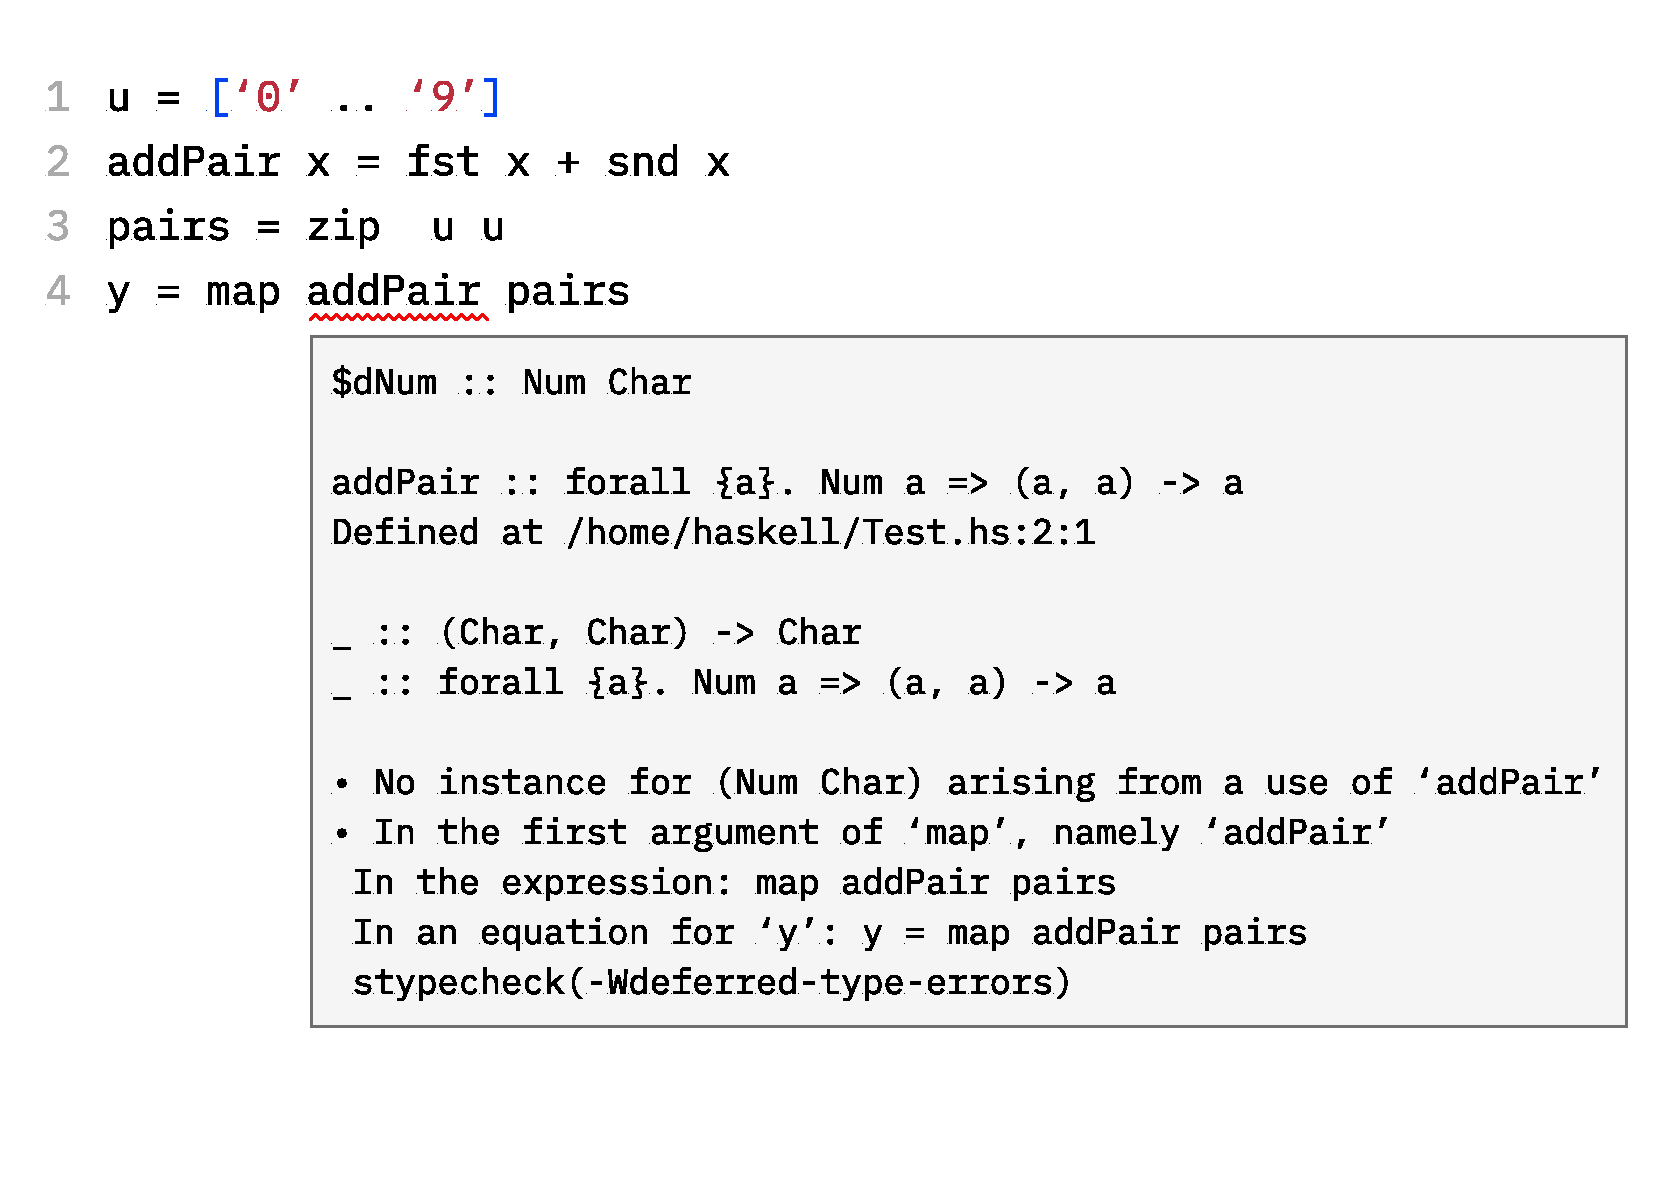
\includegraphics[width=\linewidth,trim=0mm 35mm 0mm 0mm]{images/add-pair-example.pdf}
    \caption[A type error displayed in Visual Studio Code and the Haskell Vscode extension]{
    A type error displayed in Visual Studio Code\cite{Microsoft_undated-hs} \todo{Missing citation} and the Haskell Vscode extension\cite{noauthor_2023-ot}.
The expression \texttt{addPair} is blamed for causing the type error. This may not match the programmers' intention. 
    }
    \label{fig:motivation-example}
\end{figure}

\textbf{Traditional type errors show only limited location}
Haack and Wells~\cite{Haack2004-fr} noted that ``\textit{Identifying only one node or subtree of the program as the error location makes it difficult for programmers to understand type errors. To choose the correct place to fix a type error, the programmer must find all the other program points that participate in the error.}'' The type error in Fig.~\ref{fig:motivation-example} can be fixed in multiple locations. For instance  replacing \texttt{['0'..'9']} on line 1 with \texttt{[0..9]}, or replacing \texttt{fst x} and \texttt{snd x} on line 2 with \texttt {read (fst x)} and \texttt{read (snd  x)}. In the type error message, only the \texttt{addPair} expression on line 4 was blamed.  In this small example, the whole context is visible, but it can become problematic in large programs where the lines contributing to the type error are far apart in the source code.

\textbf{Traditional type errors are biased}
A common form of bias happens when a type error is reported in one expression, but it can occur in multiple other expressions as well. In Fig.~\ref{fig:motivation-example}, the error message arbitrarily focuses on only \texttt{addPair}, while ignoring that the literals in the definition of \texttt{u} may be incorrect. %Technically, this results from the side effect of different unification orders of the internal type-checking technique and has no bearing on what the programmers think and expect. 
Another form of bias is that traditional type errors are often framed as conflicts between \texttt{Expected type} and \texttt{Actual type}. This framing is standard practice in most typed languages. However, what is \texttt{expected} and what is \texttt{actual} are a side effect of different unification orders rather than the intention of the programmer. In both forms, the error message may lead programmers to falsely believe the validity of parts of code and wrongly accuse others.

\textbf{Traditional type errors give poor explanations}
When the compiler rejects a program, the internal state of type checking is the result of a complex computation. But the details of this process are hard to explain to users and are usually not reported by compilers. For the typical type error shown in Fig.~\ref{fig:motivation-example}, the evidence for the type error is gathered from the previous declarations. These have to be rediscovered by programmers using less rigorous methods. 

\subsection{Design Goals of \chameleon{}}
Based on the limitations of traditional type errors, we give the following design requirements for \chameleon{}:

\noindent\textbf{Show} all the possible locations where the type error happened or could have happened.

\noindent\textbf{Explain} type errors avoiding jargon and internal constructs of the type checker.

\noindent\textbf{Do not presume} which expression is to blame for the type error based on the order of computation or which possible type for an expression is `actual' or `expected'.


\section{Chameleon IDE} \label{chameleon}
\begin{figure*}
    \centering
    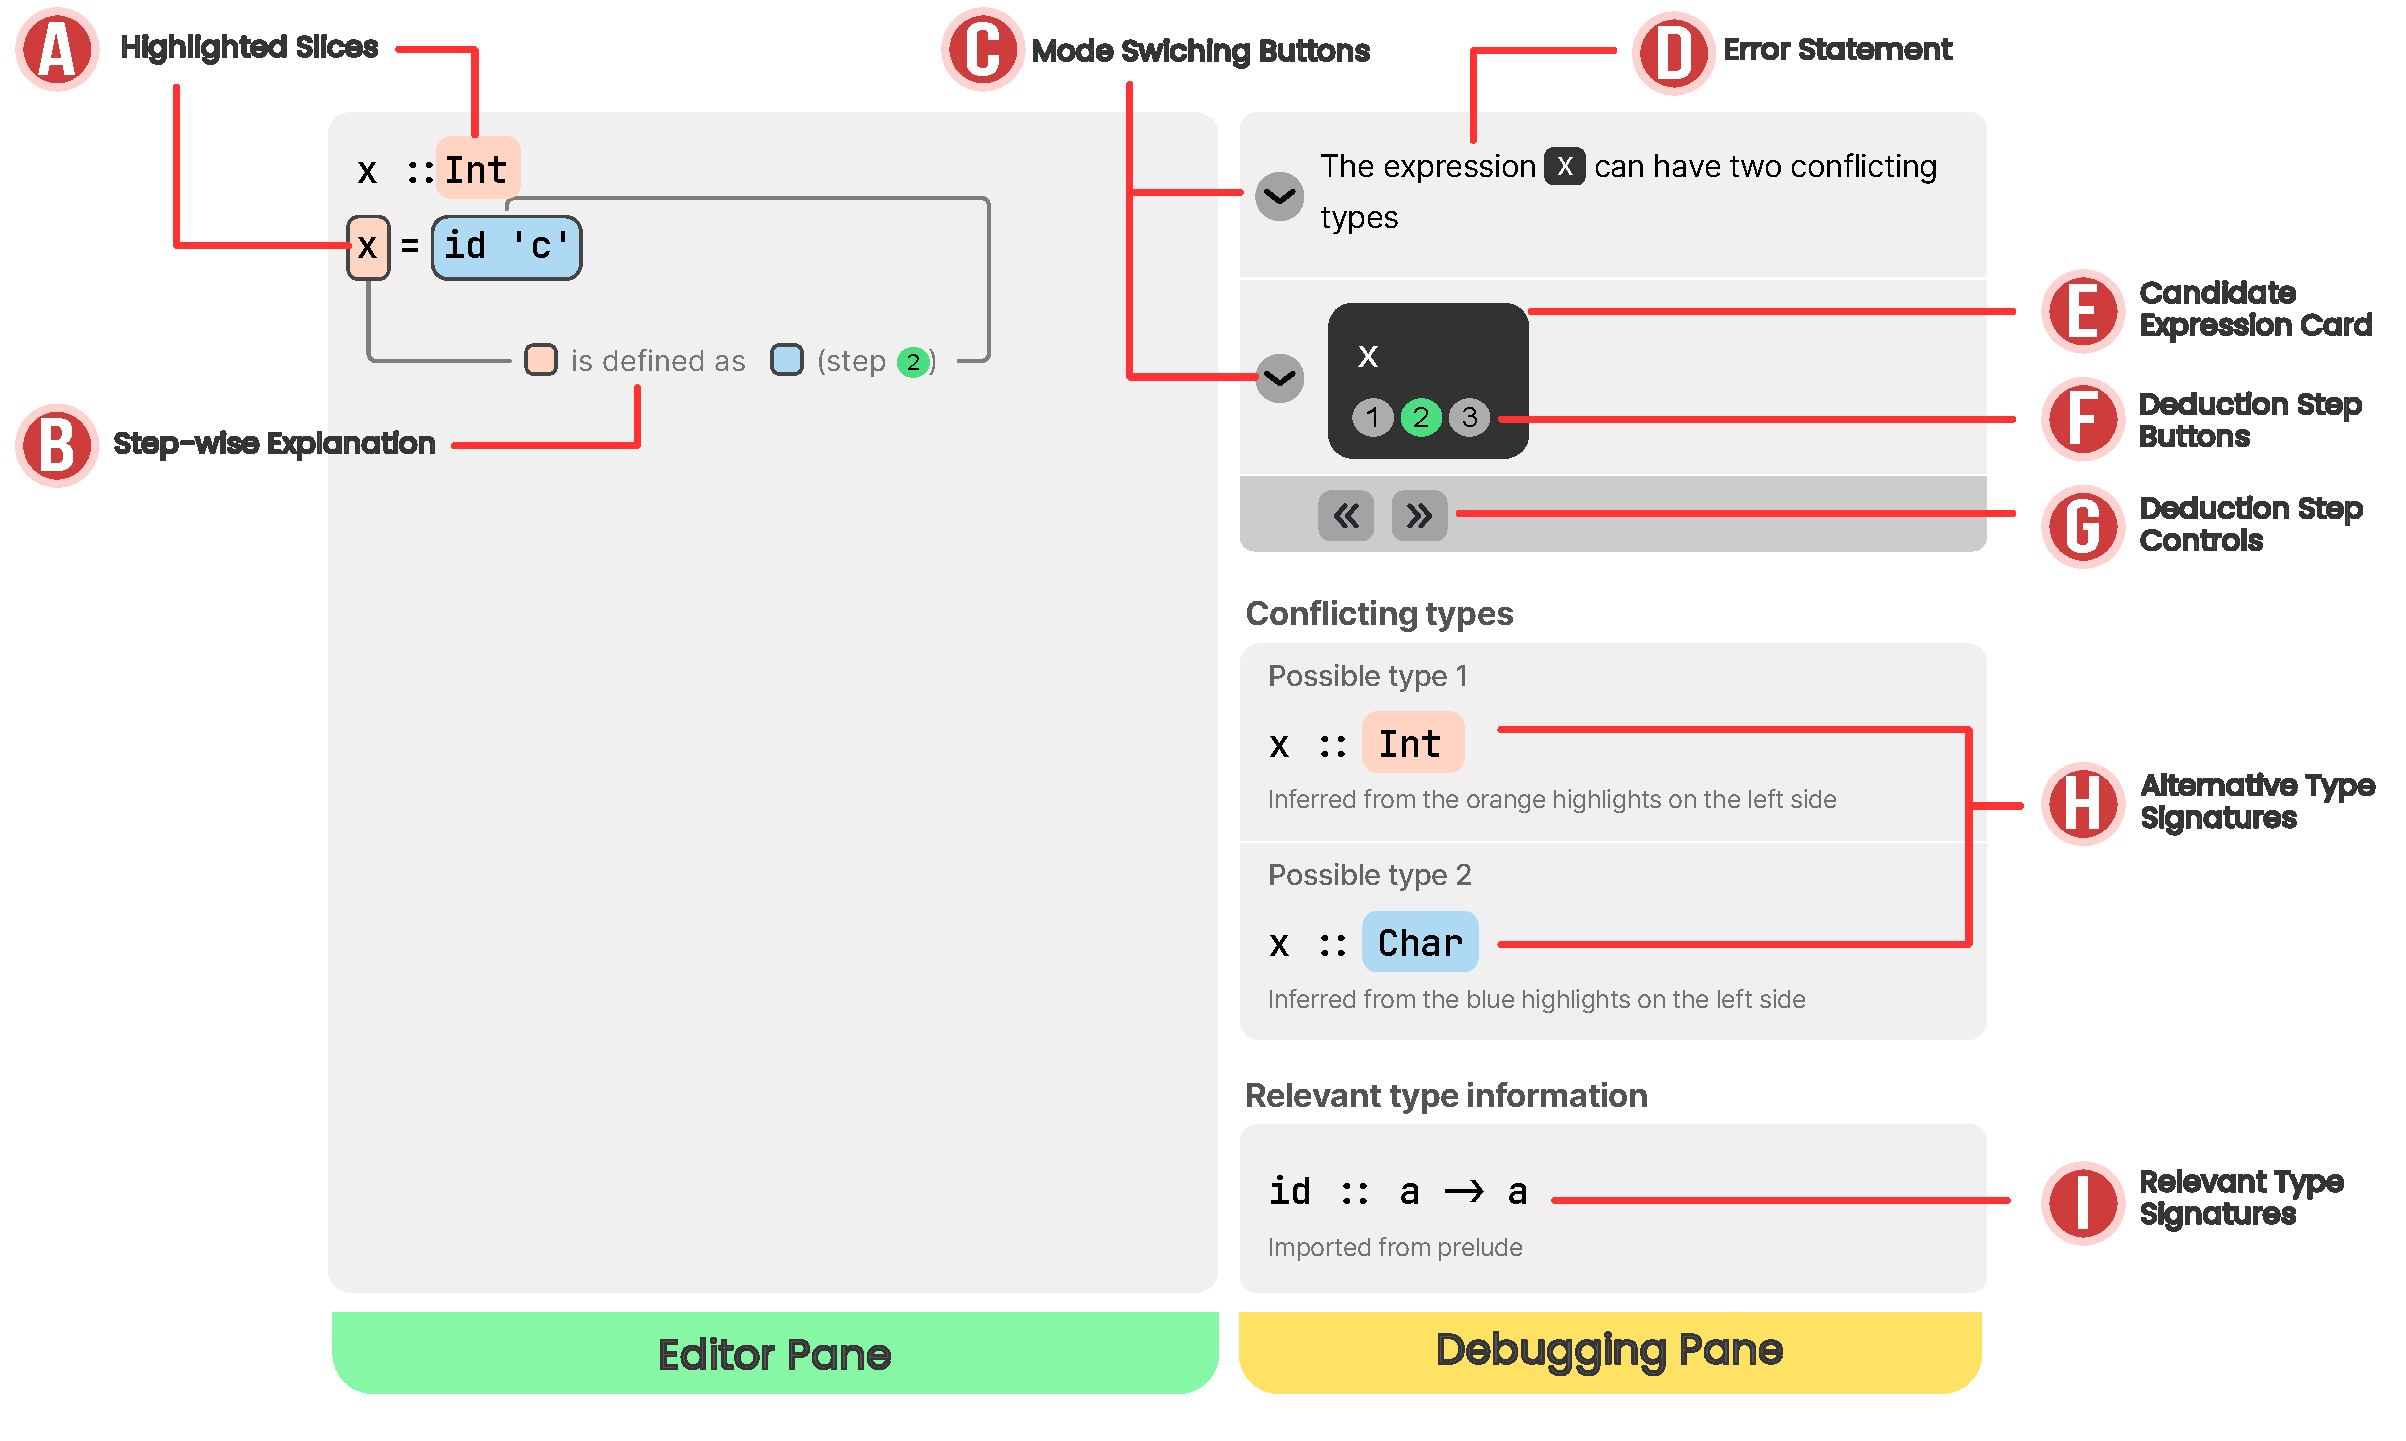
\includegraphics[width=\textwidth, trim=0mm 10mm 0mm 0mm]{images/atonomy.pdf}
    \caption[The anatomy of \chameleon{}]{
        \textbf{The anatomy of \chameleon{}.}
        The editor pane (left) is similar to a traditional code editor. Fragments of source code may have a highlight
        color (A). Additionally, an explanation layer (B) displays if deduction steps are enabled. The debugging pane contains three blocks. First, the error statement block contains an error statement (D), optionally, a list of candidate expression cards (E), a list of deduction steps (F), and a control bar (G) to increment/decrement deduction step. Second, the conflicting types block shows two alternative types (H). Third, the relevant type information block shows additional information (I) that may help understand type errors.
    }
    \label{fig:anatomy}
\end{figure*}


\chameleon{} comprises two parts: a type inference engine and a novel interactive debugging interface. 
% This separation of concerns allows us to (1) adapt \chameleon{} into multiple front ends, such as IDE extensions, desktop applications, and web applications; and (2) reuse the debugging interface for different programming languages by replacing the back-end type inference engine. 
The debugging interface is designed from the ground up; the type inference engine is a re-implementation of the original Chameleon with several novel improvements, as described in Section \ref{sec:typeinferenceengine}.

% \todo{I wonder about a high level overview diagram of tool / usage of tool, then the details of each component?}

% \todo{Can you use this example in Motivating Example sectoon (see my comment above) then use it to explain tool in this section?  Make sense?

% Is this example too simple...?}

\subsection{The Debugging Interface}

The \chameleon{} debugging interface provides three main features to visualize and explain type errors.

% the relation between the error statement and locations in code and to explore the explanation of each error location given by the type inference engine. 
%Further, programmers  can turn on and off features to suit their preferences and debugging needs.


\paragraph{Type compare tool} \label{sub:type-compare}
% In designing \chameleon{}, we want to argue against the practice of reporting type errors as the conflicts between \texttt{Expected type} and \texttt{Actual type}. Technically, the two alternatives are merely the side effect of different unification orders of the internal type-checking technique and have no bearing on what the programmers think and expect. 

The type compare tool shows conflicting types in different colors, each type associated with one or more error locations highlighted in a matching color (Fig.~\ref{fig:compare}).  
%The type error must be fixed by modifying at least one of these locations. 
%Error locations are highlighted with the matching color of the conflicting types. The type compare tool is useful to quickly bisect the type error. 
If the programmers know the expression's intended type (they usually do), they will be able to eliminate half of the possible locations. 
%To make this bisecting effect more pronounced, a user can hover over one of the possible types and only show the relevant locations that contribute to that type. 
A hover interaction over one of the possible types facilitates such bisection, causing only the relevant locations that contribute to that type to be highlighted. 
%This is a convenient way to put the error \emph{under the spotlight}.


\begin{figure}
    \centering
    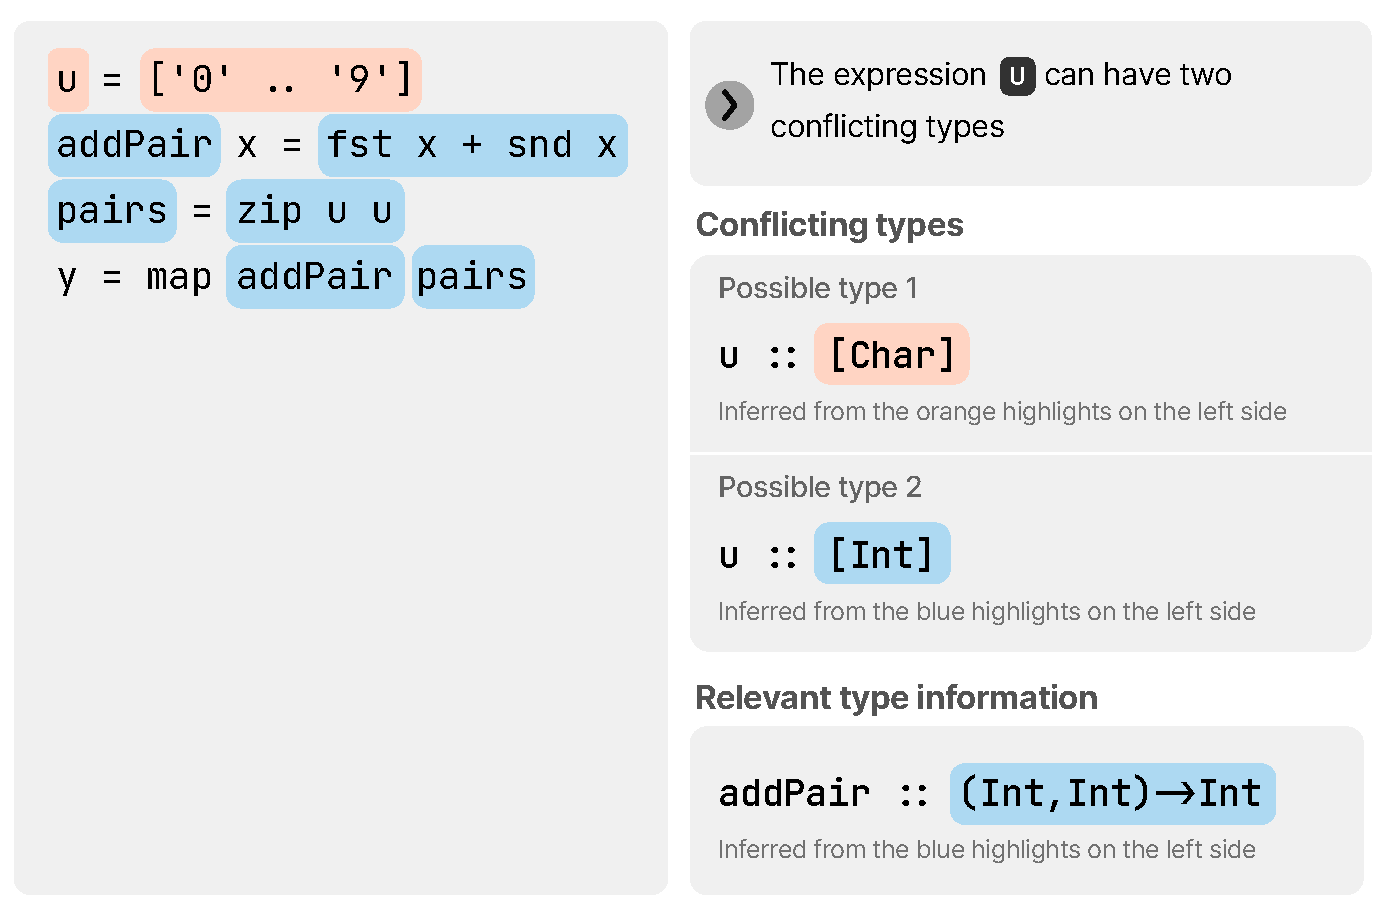
\includegraphics[width=\linewidth, trim=0mm 10mm 0mm 0mm]{images/intro-compare-2.pdf}
    \caption[\chameleon{} with type compare tool enabled]{
        \textbf{\chameleon{} with type compare tool enabled}. \chameleon{} identified the conflicting types for the expression \texttt{u} and associated the relevant locations with each type. Compare the output with the traditional type error message in fig. \ref{fig:motivation-example}.
}
    \label{fig:compare}
\end{figure}

\begin{figure}
    \centering
    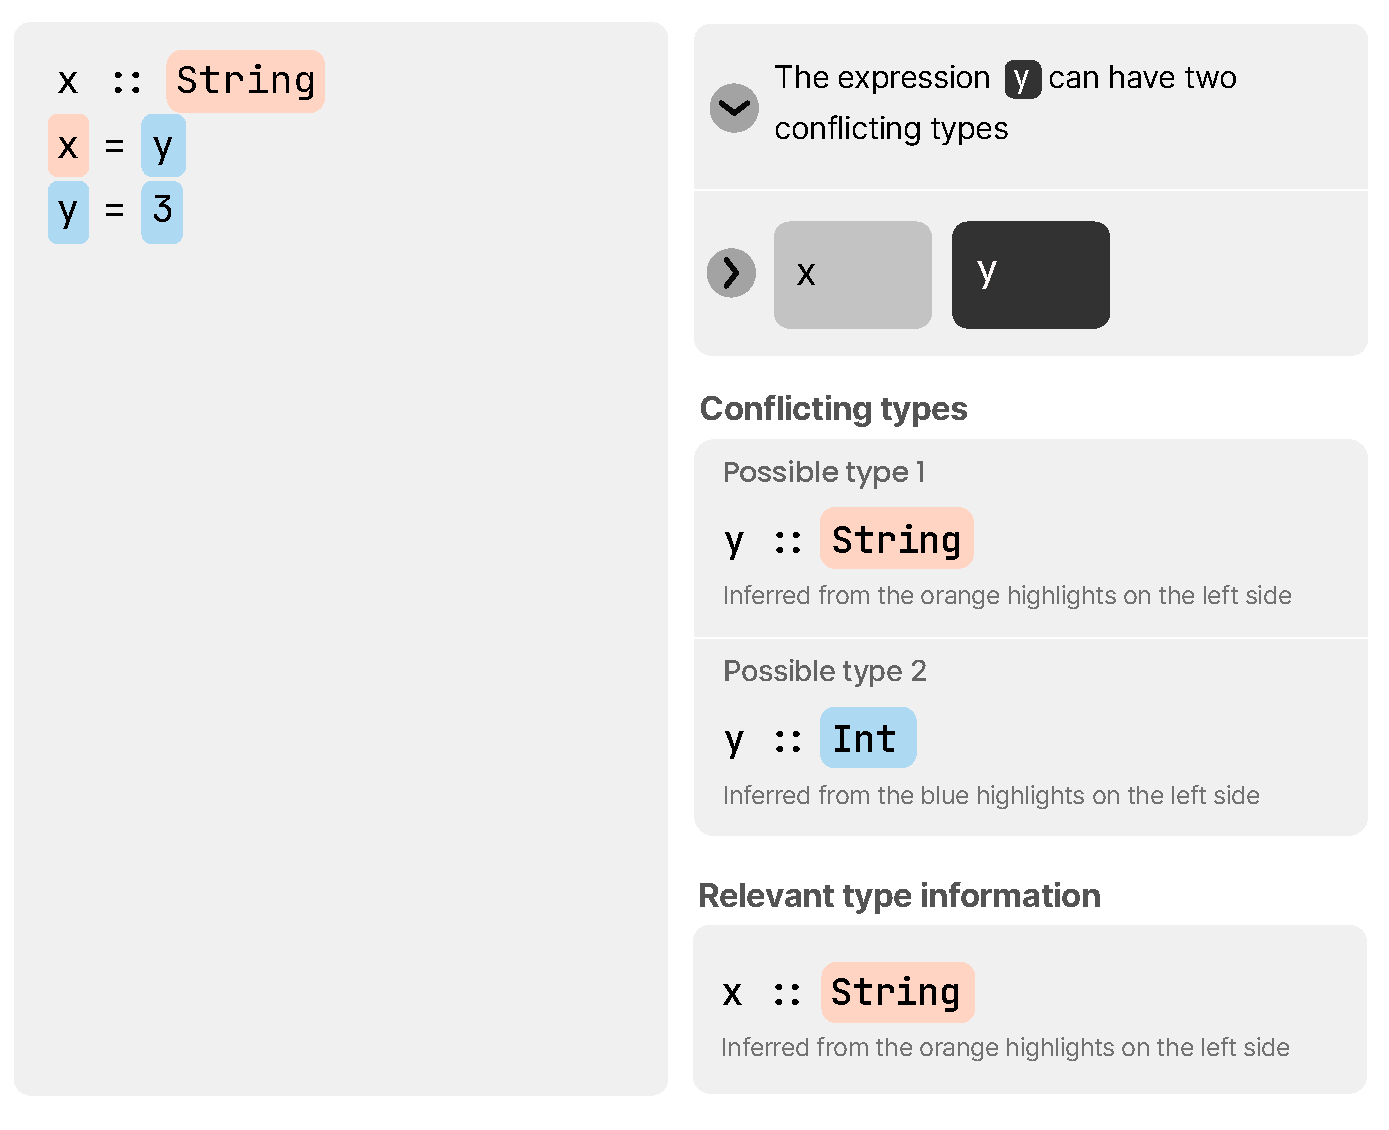
\includegraphics[width=\linewidth, trim=0mm 10mm 0mm 0mm]{images/intro-candidate.pdf}
    \caption[\chameleon{} with candidate expression cards enabled.]{
        \textbf{\chameleon{} with candidate expression cards enabled.}
        Indicates the type error can occur in the definition of \texttt{x} or \texttt{y}.
    }
    \label{fig:expression}
\end{figure}


\begin{figure}
    \centering
    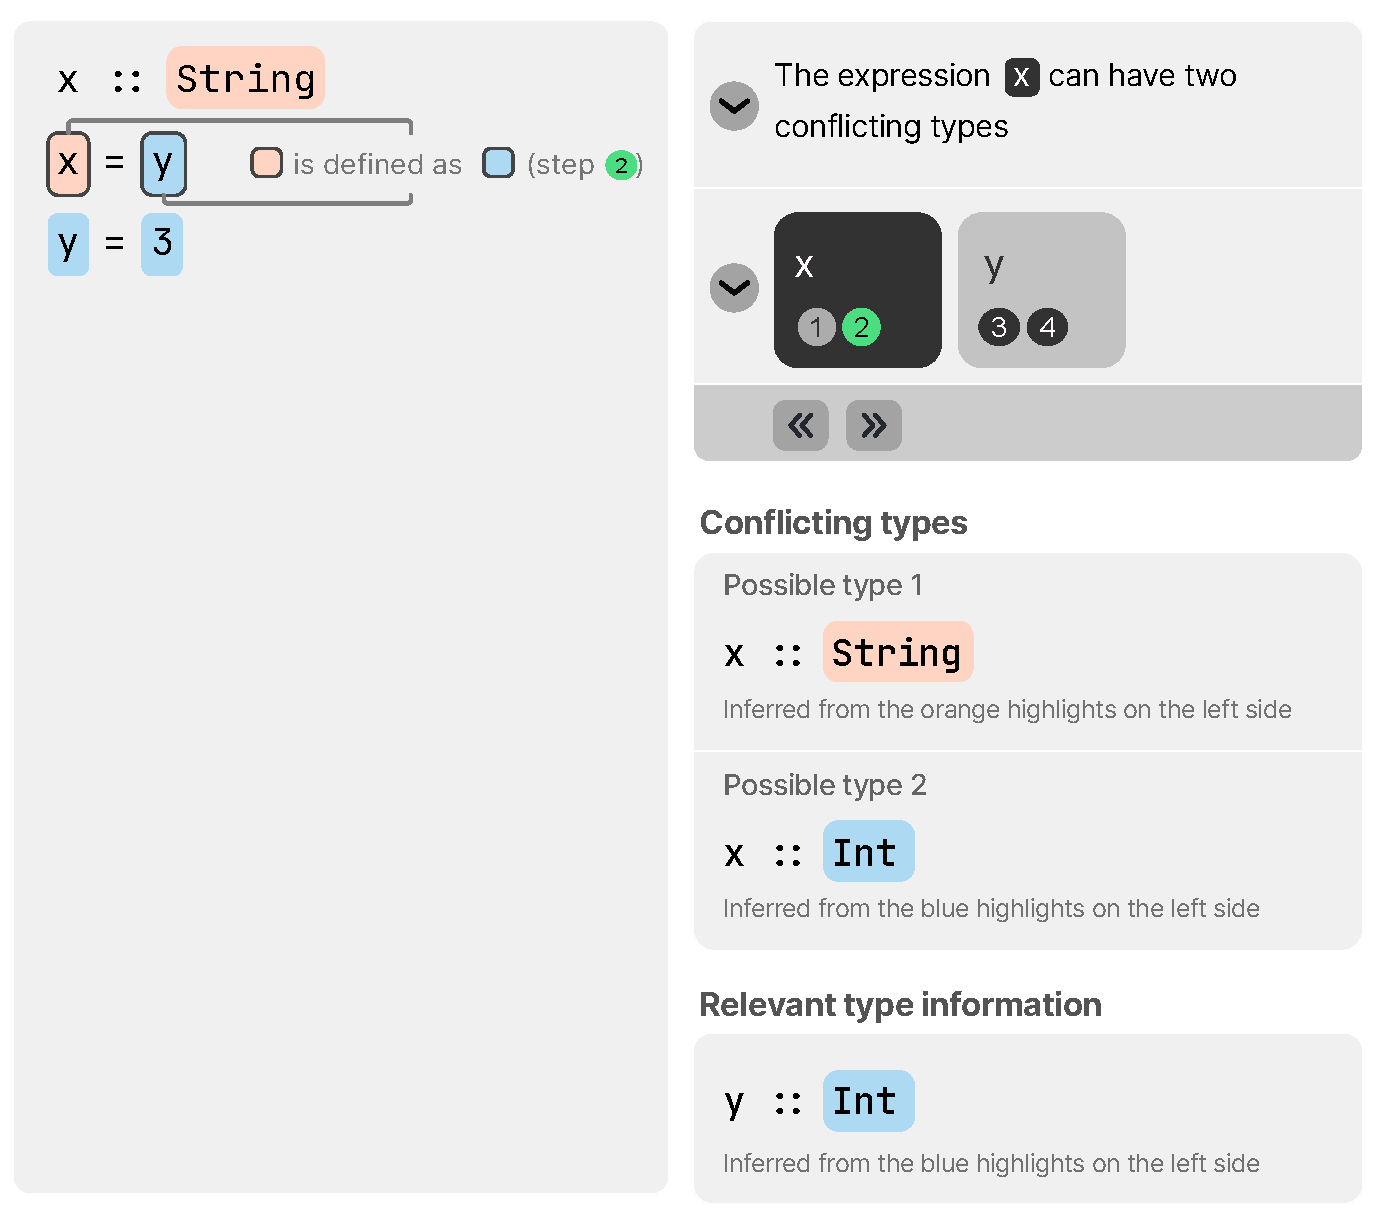
\includegraphics[width=\linewidth, trim=0mm 10mm 0mm 0mm]{images/intro-deduction.pdf}
    \caption[\chameleon{} with deduction steps enabled]{
        \textbf{\chameleon{} with deduction steps enabled.}
        \chameleon{} explains the type error in four steps. In the screenshot, the active step is step 2, where \chameleon{} shows that the expression \texttt{x} and \texttt{y} should have the same type. 
    }
    \label{fig:deduction}
\end{figure}



\paragraph{Candidate Expression Cards}  \label{sub:candidate-expression}


% We propose candidate expression cards to make it clear to the user that there are multiple ways to resolve a type conflict. By contrast,  standard compiler error messages such as those of GHC arbitrarily focus the users' attention on only one candidate expression, e.g.\ ``\textit{Couldn't match expected type ‘Char’ with actual type ‘Bool’ in expression x}" where x is the candidate expression. In practice, this candidate expression often does not match programmers' intention (Fig. \ref{fig:single-candidate}).  
A candidate expression is an expression that can be inferred to have two conflicting types. 
When a type error is detected, \chameleon{} provides a list of all candidate expressions, and programmers are free to choose the problem to resolve by clicking on one candidate expression card. In the example shown in Fig. \ref{fig:expression}, \texttt{x} and \texttt{y} are both candidate expressions. Fixing either type error can make both expressions well-typed.


% This feature can be effective in resolving the problem that traditional tools tend to report errors that happened in source code from third-party libraries. With candidate expression cards, a programmer can freely change the context of the type error to the user-defined variables and functions to gain a better understanding of why their own code does not match the library code instead of the other direction.


Programmers select a candidate expression card by clicking on one card. Once a card is selected, the information in the conflicting types block changes to reflect the change of candidate expression. In the editor pane, some error locations change highlight colors based on the updated candidate expression. Alternatively, programmers can preview the change of a candidate expression by hovering on one card. The hover effect is reverted once the cursor moves away. 


\paragraph{Deduction steps}  \label{sub:deduction-steps}

% Deduction steps are motivated by the lack of explaining why the program has type errors. When the compiler rejects a program, it dumps the internal state of type checking.  This information may be a result of complex computing but this process is not reported by compilers. For a typical type error shown in Fig. \ref{fig:ghc-error-example}, clearly, the evidence for the type error is gathered from the previous two declarations. These have to be rediscovered by the programmers again, using harder and less-sound methods. 

% \begin{figure}
%     \centering
%     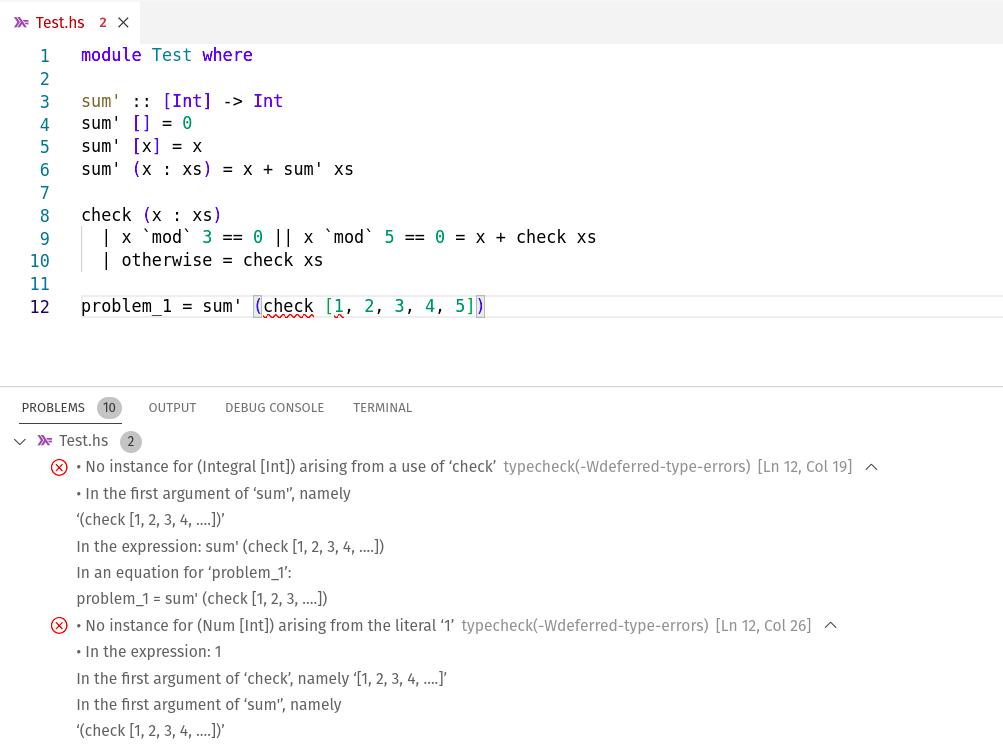
\includegraphics[width=\linewidth]{images/ghc-error-example.png}
%     \caption{
%         }
%     \label{fig:ghc-error-example}
% \end{figure}

Deduction steps allow programmers to explore all the error locations one at a time (Fig. \ref{fig:deduction}). Steps are shown as a list of sequentially  numbered circular buttons (step buttons) and an explanation layer in the editor window. In the explanation layer, the two locations under examination are outlined, and a line is drawn to connect these two locations. This line is accompanied by a human-readable text explanation of their semantic connection. Programmers are free to activate any step. The active step is shown in green. When activating a step, some highlights switch color. The message in the explanation layer changes accordingly. A program in Fig. \ref{fig:deduction} generates a list of steps shown in Fig. \ref{fig:step-interface} left.


Programmers can use mouse and keyboard shortcuts to increment or decrement the step number or jump to any step. Programmers resolve type errors by navigating through all the deduction steps and verifying whether each explanation aligns with their intention. Eventually, they will find a step that does not match, and the type error can be fixed by modifying one of the two outlined locations.

\begin{figure}
    \centering
    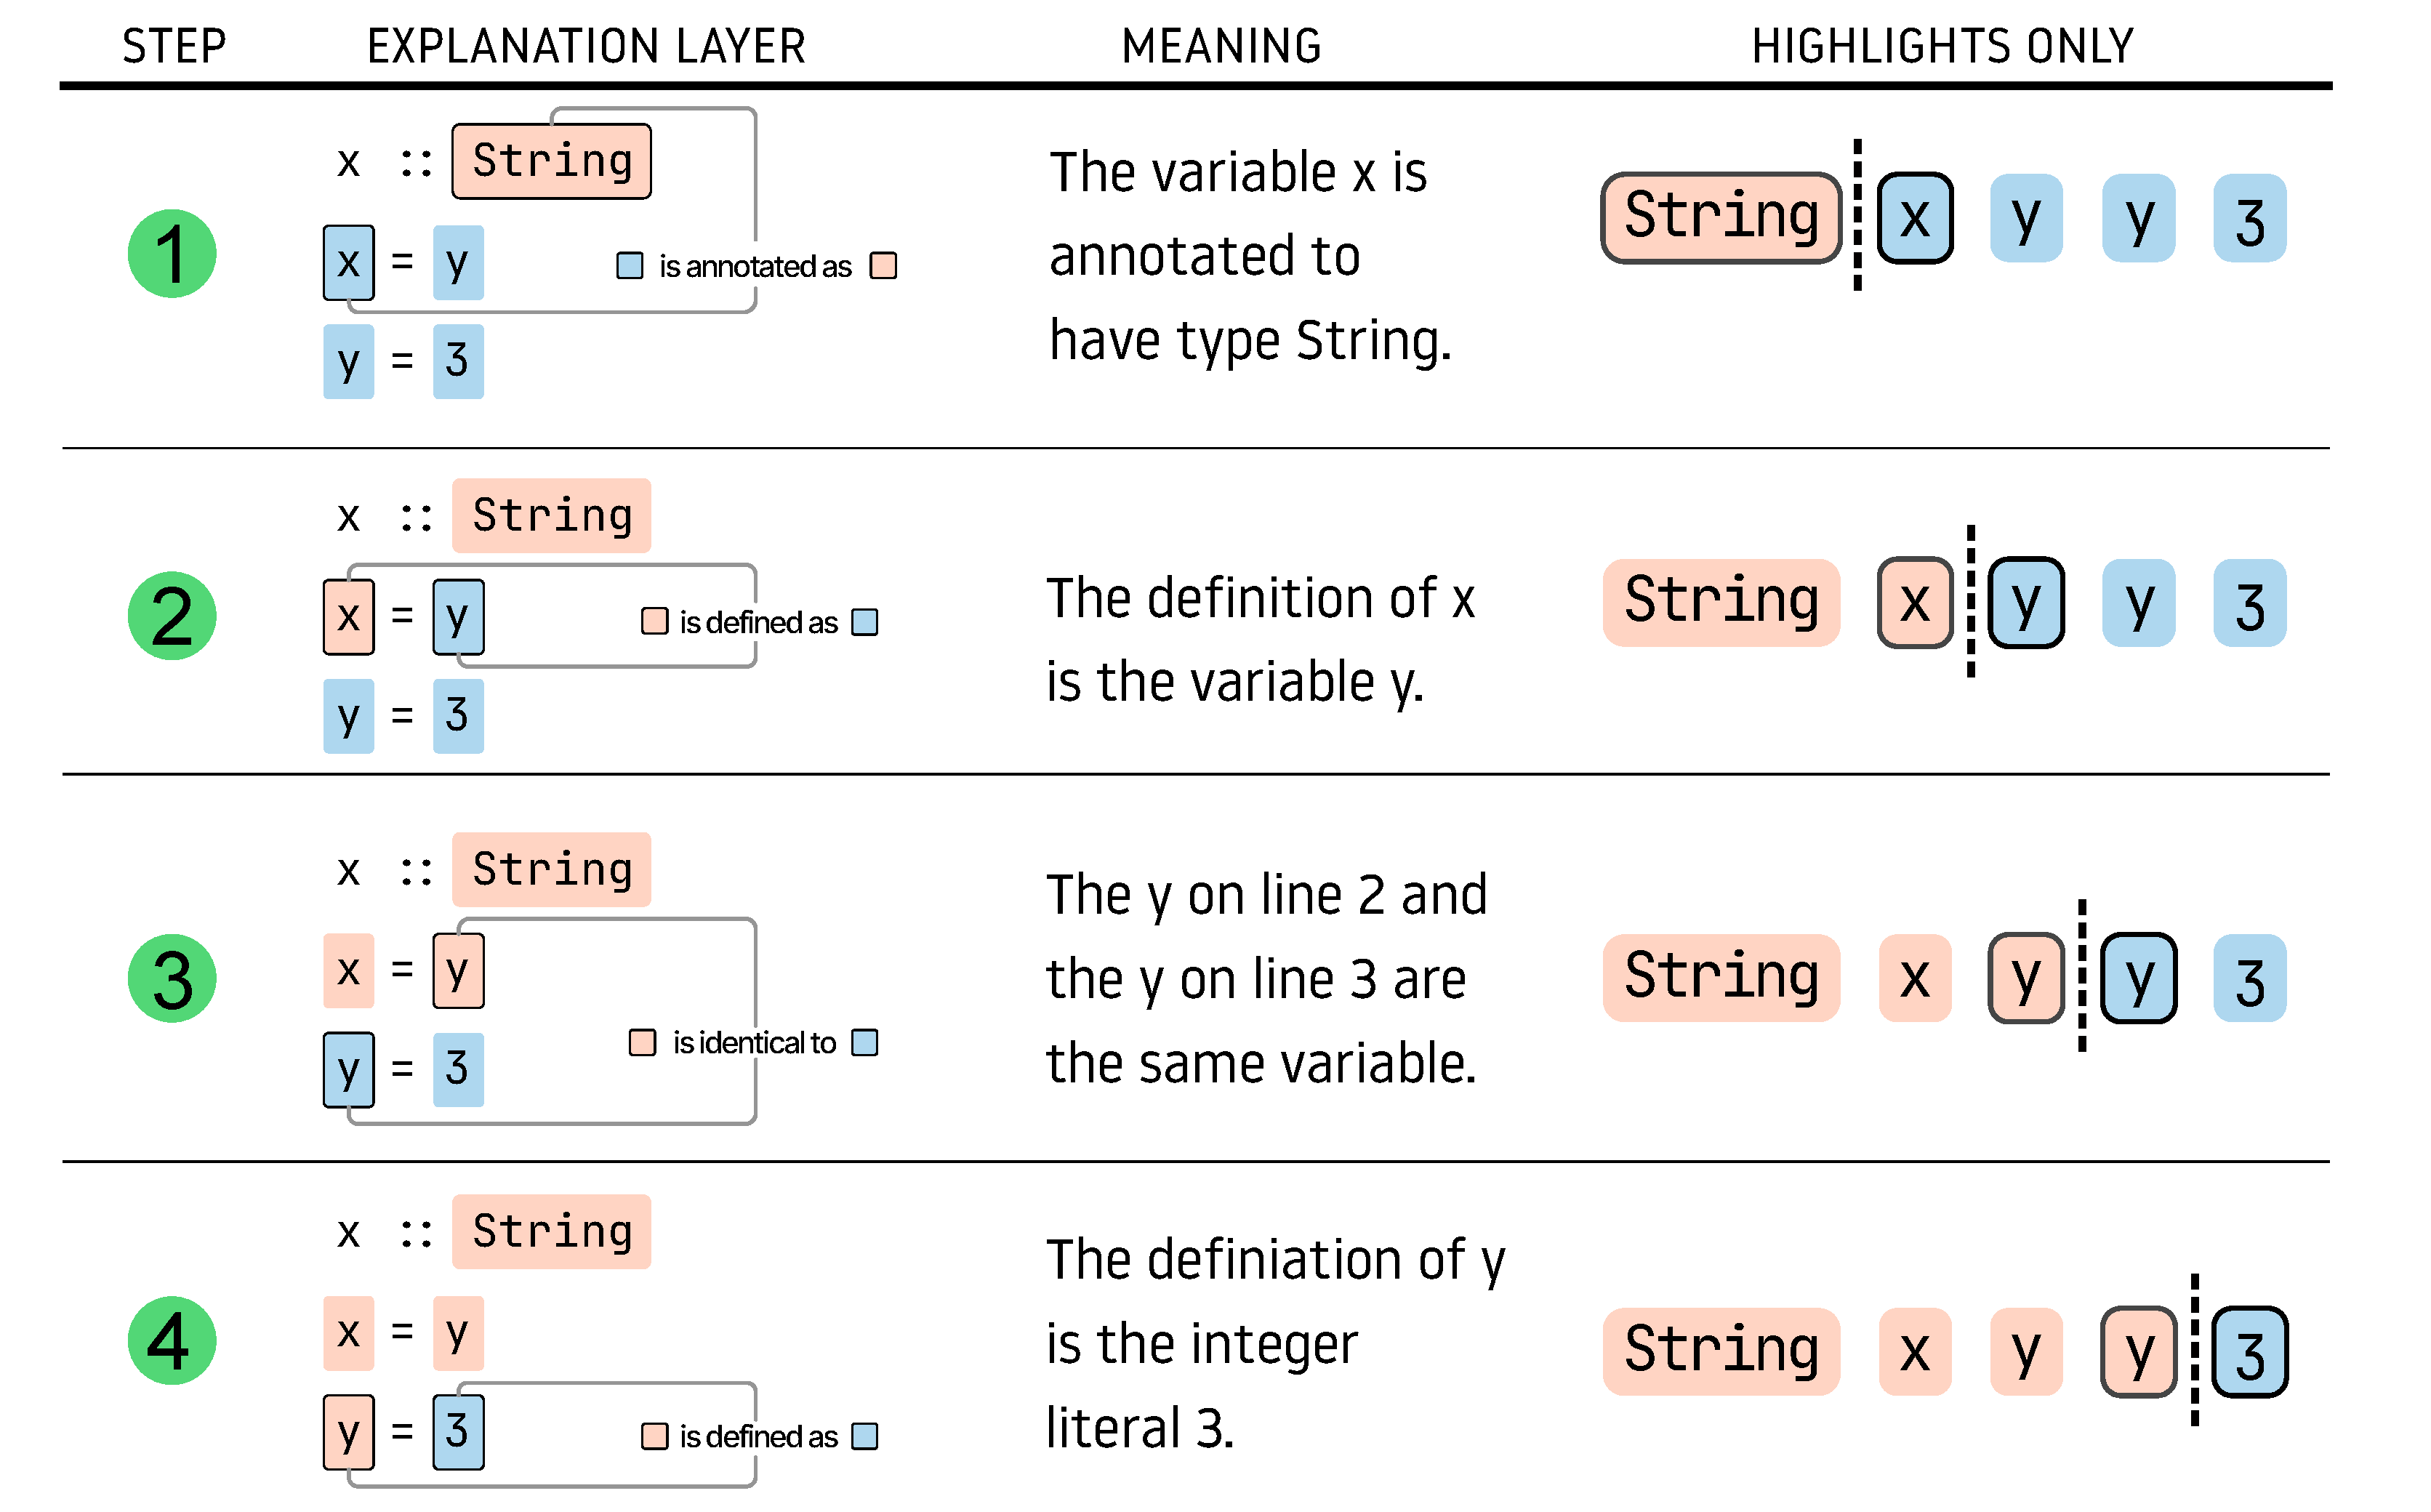
\includegraphics[width=\linewidth, trim=0mm 0mm 0mm 0mm]{images/step-explain.pdf}
    \caption[Deduction steps if they are shown all at once]{
Deduction steps if they are shown all at once. In practice, steps are shown one at a time. Programmers increment or decrement the step number using the step control bar (Fig. \ref{fig:anatomy}-G) or by directly clicking on a step button (Fig. \ref{fig:anatomy}-F). To increment or decrement the deduction step can be intuitively thought of as moving the position of the \textit{splitting point} (dotted lines) where the blue and orange highlights divide.
        }
    \label{fig:step-interface}
\end{figure}

Internally, deduction steps are different ways to divide the error locations into two  groups, denoted by the two colors. Each color infers a different type of the candidate expression. Each increment/decrement of the step changes the splitting point (dotted lines in Fig.~\ref{fig:step-interface}) of the two colors.


\paragraph{Multiple Modes}

Nielson pointed out  that the two most important issues in designing for usability are understanding the users' tasks and the differences in users \cite{Jakob_Nielsen1994-gd}. From analyzing how users use \chameleon{}, we realized that the ideal debugging interface should adapt to the specific programmer and programming task. There are cases where a programmer wants the debugger to simply ``show the answer", and others to dive deeper into the problem domain and search for the optimal solution. To accommodate the need to customize the level of information density and granularity of control, \chameleon{} provides three modes: basic, balanced, and advanced. Programmers can switch between modes by clicking on the mode switching toggles (Fig. \ref{fig:anatomy}-C). The features accessible from different modes are summarized in table~\ref{tab:chameleon-features}.%shown in table~\ref{tab:chameleon-features}.

\begin{table}
    \centering
\begin{scriptsize}
\begin{center}

    \begin{tabular}{ l l  }
     \textit{Mode} & \textit{Features} \\ \hline
     Basic Mode & Type Compare Tool \\ \hline
     Balanced mode & Type Compare Tool \\
     & Candidate Expression Cards \\  \hline
     Advanced mode & Type Compare Tool \\
     & Candidate Expression Cards \\
     & Deduction Steps \\
    \end{tabular}
    \end{center}
\end{scriptsize}
    \caption{\chameleon{} modes and features}
    \label {tab:chameleon-features}
\end{table}


\subsection{The Type Inference Engine}
\label{sec:typeinferenceengine}

Chameleon was originally a command-line tool developed in the early 2000s to improve type error reporting %and introduced a design for interactive type debugging 
for the Haskell programming language.
Unlike traditional type errors produced by the Glasgow Haskell Compiler (GHC)~\cite{Gamari_undated-zu}, which uses a Hindley–Milner type inference system, Chameleon infers types using constraint solving. In Chameleon, constraints are generated from the source code based on typing rules. In addition, each constraint is labeled with the location where it is generated. This set of constraints is consistent if the program is well-typed and inconsistent otherwise. When a type error occurs, an efficient algorithm is used to derive a minimal subset of the constraints that still contain inconsistencies. This subset is called a Minimal Unsatisfiable Subset (MUS). From this, Chameleon can report a list of locations, using the labels of constraints that are in the MUS. Stuckey et al.~\cite{Stuckey2003-pz} showed that program locations linked to the constraints from an MUS are all relevant to the type error and must include the cause of the error.

Despite successfully borrowing the underlying ideas, we could not reuse the original implementation of Chameleon since the project language standard and libraries used were out of date. 
Our \chameleon{} implementation extends the original Chameleon approach in a number of ways.
%In addition to what Chameleon can do, a few new type inference features were added in the \chameleon{} implementation.



\paragraph{Recovering concrete types from type errors}


Using only constraints from the MUS is sufficient to locate the type error, but to recover types from type errors we need constraints from parts of the program that are irrelevant to the type error.  For instance, consider an ill-typed 2-tuple where two possible types can be assigned: \texttt{(Int, Int)} and \texttt{(Int, String)}. The types reconstructed from Chameleon may be \texttt{(a, Int)} and \texttt{(a, String)}. Although the recovered types are theoretically correct, they introduce the notation \texttt{a}, which denotes a generic type variable that can be any type, making the error message harder to understand. To solve this issue in \chameleon{}, for each constraint \texttt{c} in the MUS, we find a maximally satisfiable subset (MSS) from all the constraints that contain every other element of MUS but not \texttt{c}. These maximally satisfiable subsets, while not helpful in error localization, will produce the most concrete types, see Fig.~\ref{fig:compare-to-original}. Concrete types, such as \texttt{Int} and \texttt{String},  often provide extra information to programmers. With a type of \texttt{(Float, Float)}, programmers may want to convey a point in 2d space. However, a type of \texttt{(a, Float)} does not preserve such information.


\begin{figure}
    \centering
    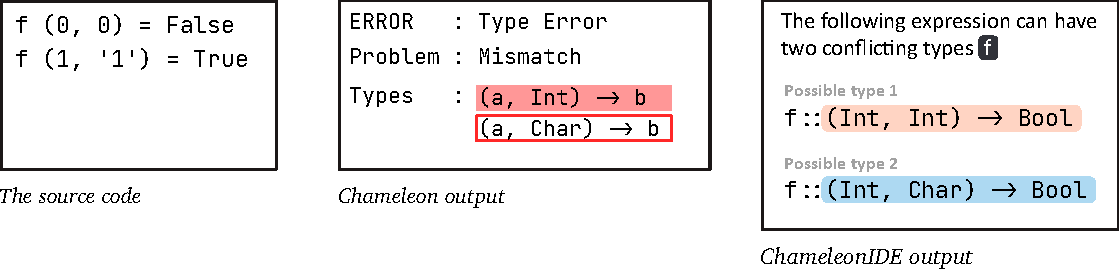
\includegraphics[width=\linewidth, trim=0mm 6mm 0mm 0mm]{images/compare-to-original.pdf}
    \caption[Comparison between original Chameleon and \chameleon{}]{
Reporting the same type error, Chameleon uses more abstract types
\texttt{Int -> a} and \texttt{Char -> a}, while \chameleon{} uses the 
concrete types (types that do not contain type variables) \texttt{Int -> Bool} and \texttt{Char -> Bool}.
    }
    \label{fig:compare-to-original}
\end{figure}

 
% If the types get too verbose for programmers to identify the conflict between the two signatures, it is always possible to mute the overlapping information and highlight the differences from the debugging front end.


\paragraph{Type error explanation}

In addition, \chameleon{} provides support for type explanation. Similar to the type explanation system  in ~\cite{Jun2002-xp},  \chameleon{} is able to produce a human-readable explanation, but for type errors. This is achieved by annotating nodes in the abstract syntax tree with constraints and the type inference rules used. We generate an inference history from constraints and accompanying annotations. 


% \begin{lstlisting} [
%     language=Haskell, caption={
%     A simple program that is ill-typed. This program generates two constraints from line 1 and one constraint from line 2.
% }, label={listing:ifelse}
% ]
% if a then b else c
% a = "True"
% \end{lstlisting}


\begin{figure}
    \centering
    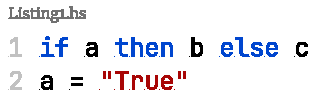
\includegraphics[width=0.4\linewidth]{images/Listing1.pdf}
    \caption[An example to illustrate constraint generation in \chameleon{}]{A simple program that is ill-typed. It generates two constraints from line 1 and one constraint from line 2. }
    \label{fig:listing1}
\end{figure}

For instance, for the program in Fig.~\ref{fig:listing1}, \chameleon{}  generates the following constraints and labels (in brackets) $T_a = Bool$ (if condition), $T_b = T_c$ (if branches), $T_a= String$  (definition). Clearly, as $T_a$ can not unify with both \textit{Bool} and \textit{String}, this program is not well typed. \chameleon{} can construct a human-readable explanation from the MUS. An example output for Fig.~\ref{fig:listing1} can be: \texttt{a} has type \texttt{Bool} because \texttt{a} is the condition of an if statement; however, \texttt{a} has type \texttt{String} because \texttt{a} is defined as the string literal \texttt{"True"}. This explanation facilitates the deduction steps (Section \ref{sub:deduction-steps}). \looseness=-1






